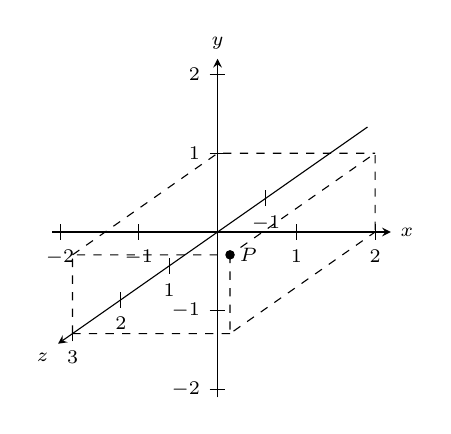
\begin{tikzpicture}[x={(1,0)},y={(0,1)},z={(-.614,-.43)},>=stealth]

\draw[->] (-2.1,0) -- (2.2,0) node [right] {\scriptsize $x$};
\draw[->] (0,-2.1) -- (0,2.2) node [above] {\scriptsize $y$};

\foreach \x in {-2,-1,1,2}
{
\draw (\x,-.1) node [below] {\scriptsize $\x$} -- (\x,.1);
\draw (-.1,\x) node [left] {\scriptsize $\x$} -- (.1,\x);
}

\foreach \x in {-1,1,2,3}
{
\draw (0,-.1,\x) node [below] {\scriptsize $\x$} -- (0,.1,\x);
}

\draw [->] (0,0,-3.1) -- (0,0,3.3) node [below left] {\scriptsize $z$};

\draw [dashed,{\colortwo}] (2,1,3) --(2,0,3) -- (2,0,0)
							(2,0,3) -- (0,0,3)
							(0,0,3)--(0,1,3) -- (2,1,3)--(2,1,0) -- (2,0,0)
							(0,1,3) -- (0,1,0) -- (2,1,0);
\filldraw [{\colorone}] (2,1,3) circle (1.5pt) node [right,black] {\scriptsize $P$}; 	
\end{tikzpicture}
